\section{Vertex-Centric Graph Index}\label{sec:storage}
\begin{figure*}
  \centering
  \begin{subfigure}[b]{0.27\textwidth}
    \centering
    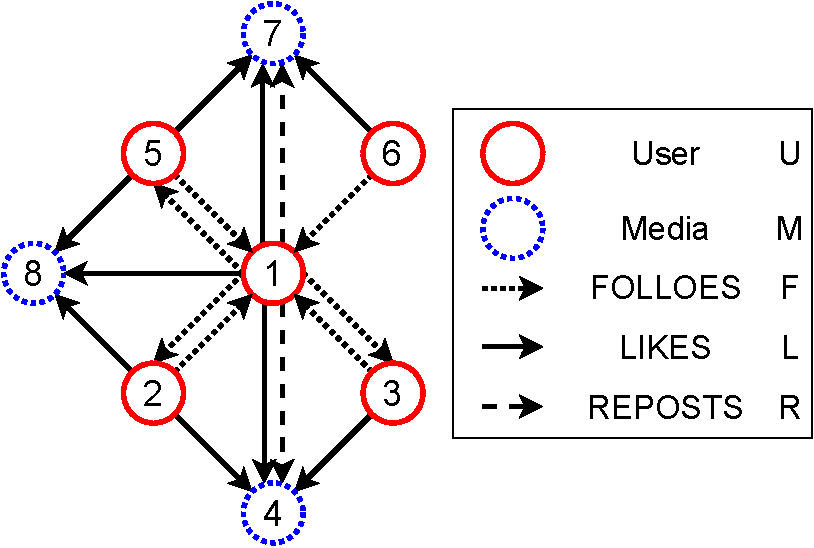
\includegraphics[scale=0.4]{img/data_graph}
    \caption{Data graph.}\label{fig:data_graph}
  \end{subfigure}
  \quad
  \begin{minipage}[b]{0.68\textwidth}
    \centering
    \begin{subfigure}[b]{\textwidth}
      \centering
      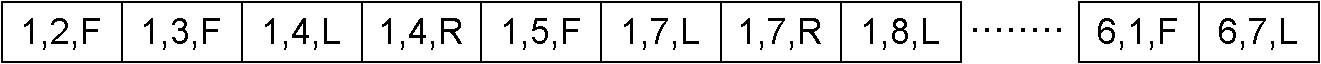
\includegraphics[scale=0.3]{img/data_edge}
      \caption{Edge List.}\label{fig:data_edge}
    \end{subfigure}
    \\
    \begin{subfigure}[b]{0.35\textwidth}
      \centering
      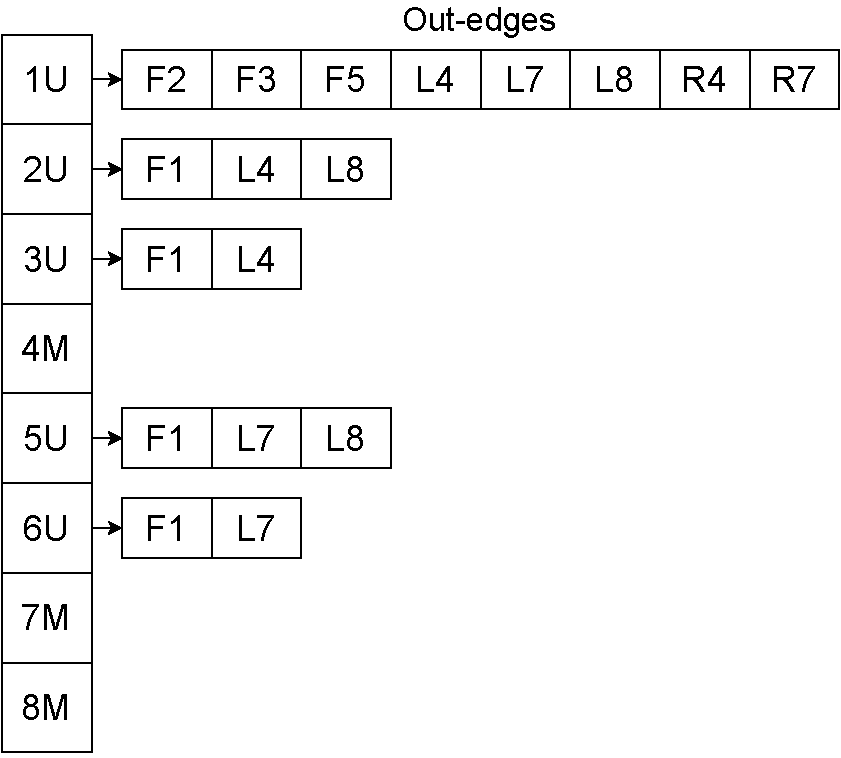
\includegraphics[scale=0.3]{img/data_row}
      \caption{Row-based.}\label{fig:data_row}
    \end{subfigure}
    \quad
    \begin{subfigure}[b]{0.2\textwidth}
      \centering
      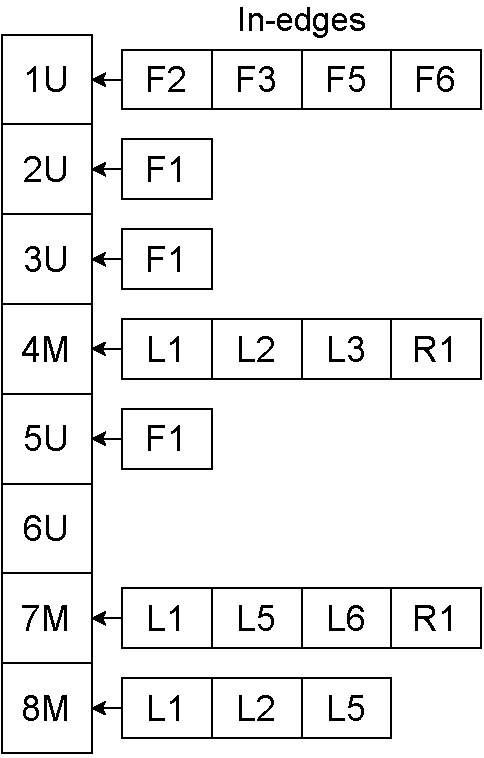
\includegraphics[scale=0.3]{img/data_column}
      \caption{Column-based.}\label{fig:data_column}
    \end{subfigure}
    \quad
    \begin{subfigure}[b]{0.3\textwidth}
      \centering
      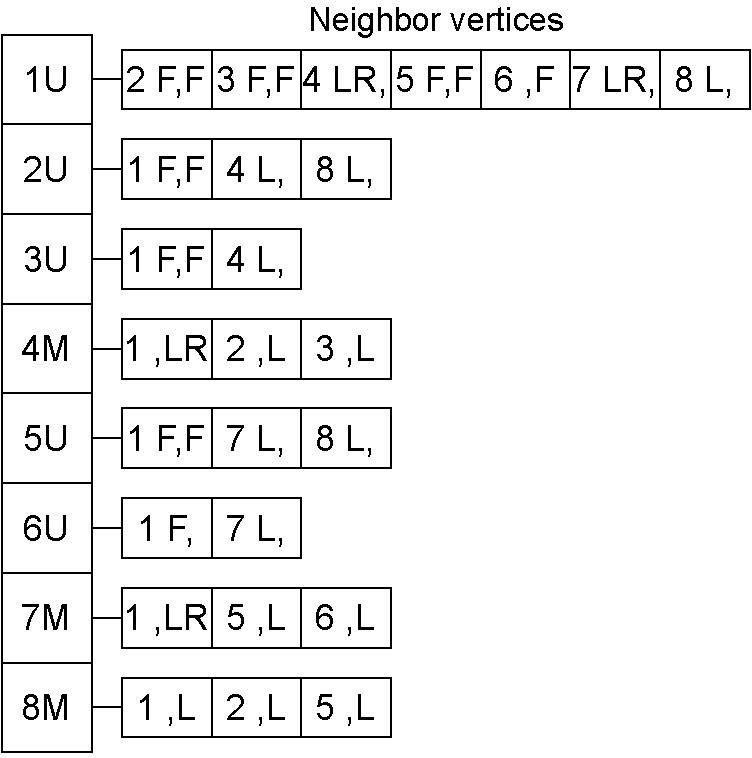
\includegraphics[scale=0.3]{img/data_vertex_centric}
      \caption{Vertex-centric.}\label{fig:data_vertex_centric}
    \end{subfigure}
  \end{minipage}
  \caption{Sample data graph and its various storage methods.}\label{img:data}
\end{figure*}
A data structure is a way to store and organize data in order to facilitates access and modifications~\cite{DBLP:books/daglib/0023376}.
The performance of a graph matching algorithm is closely related to its storing structure.
This section first shows the opportunities by studying existing graph storage methods,
then presents the design of SeqStar's graph index.

\subsection{Opportunities}
A graph can be represented by its adjacency matrix~\cite{DBLP:books/sp/BondyM08}.
Based on the accessing order of the matrix, existing graph storage methods can be categorized into three types:
\emph{edges list}, \emph{row-based} and \emph{column-based}.

Consider the sample data graph in Figure~\ref{fig:data_graph}, the \emph{edge list} format stores each edge and its corresponding source and destination vertices as a sequence (Figure~\ref{fig:data_edge}).
In the language of linear algebra, edge list is known as \emph{coordinate list (COO)}, which stores a list of $(row, column, value)$ tuples.
The neighbors of each vertex are scattered across in edge list~\cite{DBLP:conf/fast/KumarH19}, thus it is not an optimal choice for graph matching problems.

In order to access the in/out-edges of each vertex efficiently, the edge list is partitioned by the destination/source vertices.
\emph{Row-based} format can access the out-edges of a vertex efficiently.
As is shown in Figure~\ref{fig:data_row}, out-edges are grouped by the sources.
The physical structure of the row-based format can be either \emph{array based} or \emph{linked list based}.
The compressed sparse row (CSR) format stores the out-edges consecutively in an array, and use a vertex array to store the offset and size for each vertex.
Whereas the adjacency list structure stores the out-edges of each vertex separately.
Array based structure has better locality and is more suitable for graph analysis problems, whereas linked list structure are good at updates.
\emph{Column-based} format partitions the in-edges by the destinations (Figure~\ref{fig:data_column}).
Similar to the row-based format, the physical structure of column-based format can also be array/linked list based.

Graph problems are notorious for their high data access to computation ratio~\cite{DBLP:journals/ppl/LumsdaineGHB07}.
As a result, the access pattern of data graph plays an important part in the graph matching workflow.
In a property graph, 2-cycles and multiple edges may present between a pair of vertices,
e.g., in Figure~\ref{fig:data_graph}, $\circled{1} \leftrightarrows \circled{2}$ is a 2-cycle,
and there are 2 parallel edges in $\circled{1} \rightrightarrows \circled{4}$.
And the graph matching workflow needs \textbf{all} the topology information between the two vertices to determine the isomorphism (\S~\ref{sec:background_problem}).
However, existing row/column-based storage methods are designed to access \textbf{separated} out/in-edges efficiently.
And they are time consuming to check the isomorphism of multiple edges.

Consider the friendship pair $u_1 \leftrightarrows u_2$:
(1) An exploration-based graph matching algorithm will scan the out-edges for each vertex in row-based storage (Figure~\ref{fig:data_row}) to match $u_1 \rightarrow u_2$,
then check the out-edges of $u_2$ to match $u_1 \leftarrow u_2$;
Or respectively, scan \& check the in-edges in column-based storage (Figure~\ref{fig:data_column}).
The worst-case time complexity is $O(m^2)$ even though the edges are stored twice in both row-based and column-based methods.
\begin{proof}
  Let $d^{+}(v)$ be the out-degree of vertex $v$, and $d^{-}(v)$ be the in-degree of $v$.
  Graph theory tells us~\cite{DBLP:books/sp/BondyM08}:
  \[ \sum_{i=1}^{n}d^{+}(v_i) = \sum_{i=1}^{n}d^{-}(v_i) = m \]
  Then by Cauchy-Schwarz inequality, the time complexity $T$ of the \emph{scan \& check} (scans the out-edges, and searches the in-edges for each out-edge) algorithm has:
  \begin{align*}
    T^2 &= {\left(\sum_{i=1}^{n}d^{+}(v_i)d^{-}(v_i)\right)}^2 \\
    &\le \left(\sum_{i=1}^{n}{d^{+}(v_i)}^2\right)\left(\sum_{i=1}^{n}{d^{-}(v_i)}^2\right) \\
    &\le {\left(\sum_{i=1}^{n}{d^{+}(v_i)}\right)}^2{\left(\sum_{i=1}^{n}{d^{-}(v_i)}\right)}^2 \\
    &= m^4
  \end{align*}
  Therefore, $T = O(m^2)$.
\end{proof}
(2) A join-based algorithm will first match the decomposed edges $u_1 \rightarrow u_2$ and $u_1 \leftarrow u_2$,
store the intermediate results respectively, and finally join them together.
The join operation is still time consuming ($O(m^2)$ for nested loop join).
Moreover, useless matching results, e.g., $\circled{6} \rightarrow \circled{1}$, have to be stored as intermediate results.

Multiple edges are localized by the pair of vertices.
Ideally, the worst case time complexity to match a pair of vertices should be $O(m)$.
It is desirable the scan the graph only once to obtain the matching results.

\subsection{Vertex-Centric Storage Model}
We find that existing methods stores the in/out-edges \textbf{separately},
whereas the graph matching problem needs to access the in/out-edges \textbf{together}.
Based on the observation, SeqStar introduces a novel \emph{vertex-centric} storage model to boost the matching operation for multiple edges.

Similar to the conventional row/column based storage methods,
vertex-centric model also groups the edges by the vertices.
However, the edge topologies are stored \textbf{together} with the neighbor vertices in the vertex-centric format.
As is shown in Figure~\ref{fig:data_vertex_centric},
the data graph is partitioned by the vertices.
For each vertex $v$ in the data graph, the corresponding neighbor vertices are stored together.
Each neighbor vertex block stores the $(NID, L^{\rightarrow}, L^{\leftarrow})$, where $NID$ is the ID of the neighbor vertex $n$,
$L^{\rightarrow}$ is the set of edges pointed from $v$ to $n$, and $L^{\leftarrow}$ is the set of edges $v \leftarrow n$.
For example, the neighbor vertex block \framed{2 F,F} after vertex \framed{1U} describes the 2-cycle $\circled{1} \leftrightarrows \circled{2}$, and \framed{4 LR,} indicated the multiple edges $\circled{1} \rightrightarrows \circled{4}$.

\subsection{Global/Local Indexes}
